\documentclass{beamer}

\usepackage[ngerman]{babel}
\usepackage[T1]{fontenc}
\usepackage[utf8x]{inputenc}
\usepackage{lmodern}
\usepackage{amsmath}
\usepackage{wasysym}
\usepackage{eurosym}
\usepackage{subcaption}
\usepackage{icomma}
\usepackage{tikz}
\usepackage{booktabs}

\usetikzlibrary{shapes,arrows,positioning}
\renewcommand{\u}[1]{\;\mathrm{#1}}
\newcommand{\uf}[1]{\;\mathrm{#1}}

\newcounter{saveenumi}
\newcommand{\seti}{\setcounter{saveenumi}{\value{enumi}}}
\newcommand{\conti}{\setcounter{enumi}{\value{saveenumi}}}

% \usepackage{handoutWithNotes}
% \pgfpagesuselayout{3 on 1 with notes}[a4paper,border shrink=5mm]

\usetheme{Madrid}
\usefonttheme{serif}

%\AtBeginSection[]{
%  \begin{frame}
%  \vfill
%  \centering
%  \begin{beamercolorbox}[sep=8pt,center,shadow=true,rounded=true]{title}
%    \usebeamerfont{title}\insertsectionhead\par%
%  \end{beamercolorbox}
%  \vfill
%  \end{frame}
%}

\title[Schubvektorsteuerung]{Entwicklung einer Modellrakete mit Schubvektorsteuerung}
\date[2018--02--11]{Göttingen, 11. Februar 2018}
\author[Oliver Arend, Solaris-RMB e.V.]{Oliver Arend\inst{1}}
\institute[]{
\inst{1}Solaris-RMB e.V.
}

\tikzstyle{block} = [draw, rectangle, minimum height=2em, minimum width=2em]
\tikzstyle{sum} = [draw, circle]
\tikzstyle{input} = [coordinate]
\tikzstyle{output} = [coordinate]
\tikzstyle{pinstyle} = [pin edge={to-,thin,black}]

\begin{document}

\frame{\maketitle}

\begin{frame}{Übersicht}
\tableofcontents
\end{frame}

\section{Zielsetzung}

\begin{frame}{Zielsetzung}
\begin{itemize}
\item Aktiv stabilisierte Rakete durch Schubvektorsteuerung
\item Günstige, einfach erhältliche Komponenten, z. B.
\begin{itemize}
\item Arduino
\item Modellbau-Servos
\end{itemize}
\item Einfach nachzubauen
\item Erfahrungen für größere, komplexere Raketen nutzen
\item Alle notwendigen Informationen öffentlich verfügbar machen
\end{itemize}
\end{frame}

\begin{frame}{Was bisher geschah ...}
\begin{itemize}
\item Vorführung einer Schubvektorrakete durch Wolfgang Lang beim Flugtag in Manching 2015 (und seitdem immer wieder)
\item Mehrere Iterationen für das Strukturdesign:
\begin{itemize}
\item Werkstoff? Balsa, Pappelsperrholz, CfK ...
\item Herstellung? Laserschneiden, Fräsen, ...
\item Aktueller Stand: größtenteils gefrästes Flugzeugsperrholz, teilweise 3D-Druck
\end{itemize}
\item Berechnung der aerodynamischen Beiwerte mit CFD
\item Erstellung eines einfachen regelungstechnischen Modells
\item Umsetzung in Firmware
\item Probeflug
\end{itemize}
\end{frame}

\section{Mechanik}

\begin{frame}{Einzelteile kardanische Aufhängung}
\begin{center}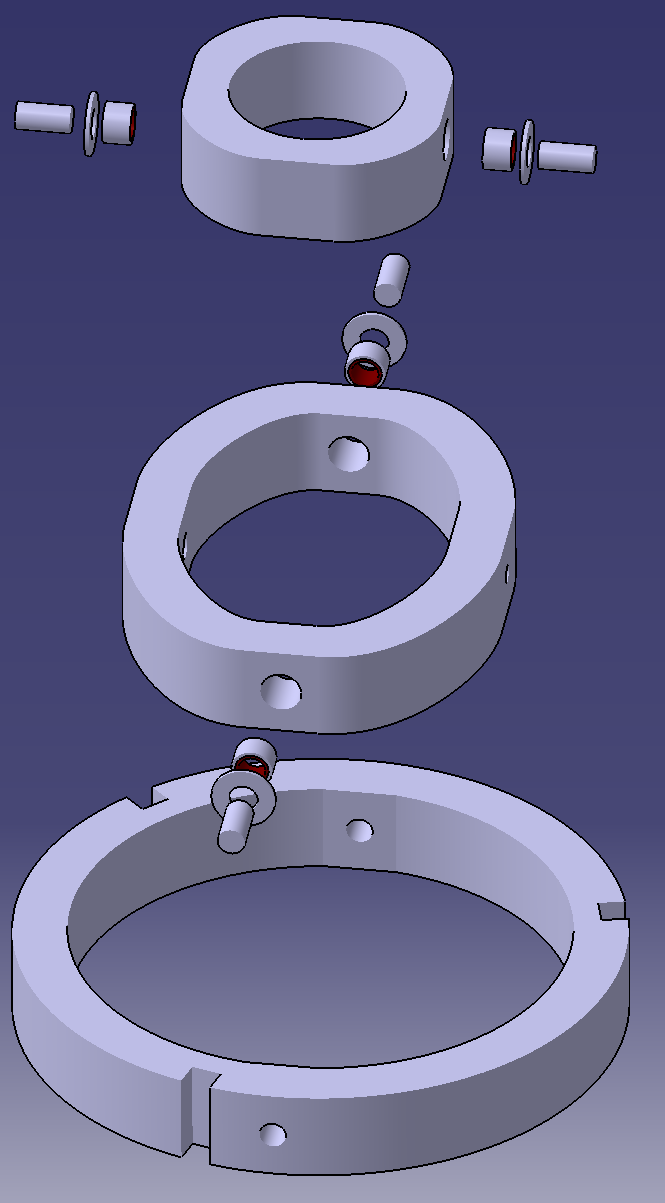
\includegraphics[height=75mm]{kardan_1.png}\end{center}
\end{frame}

\begin{frame}{Motorhalterung}
\begin{center}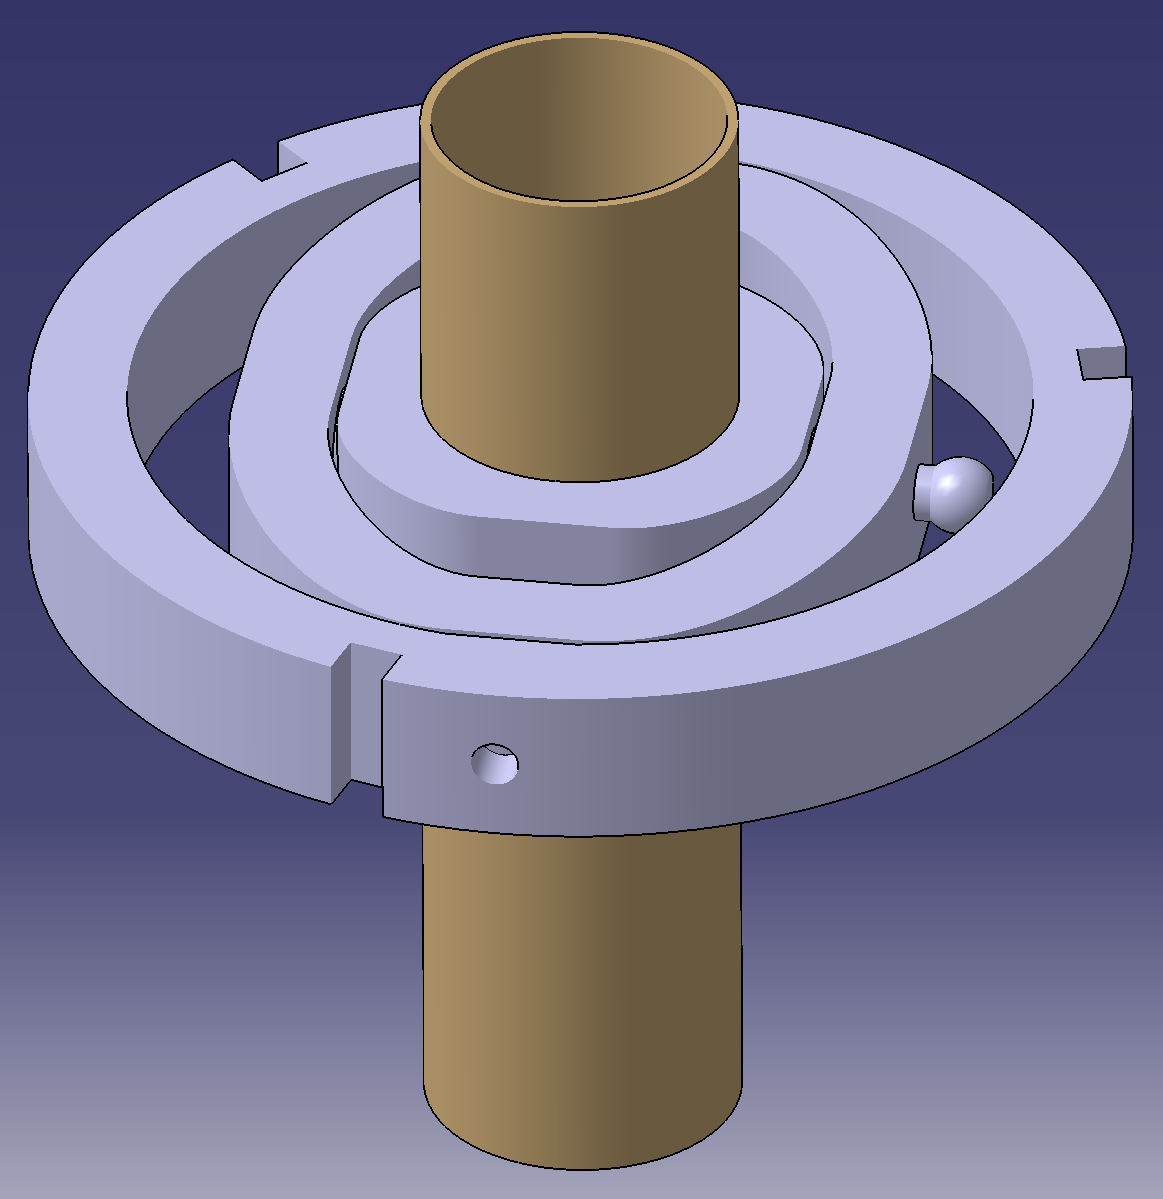
\includegraphics[height=75mm]{motor_1.png}\end{center}
\end{frame}

\begin{frame}{Servos und Halterungen}
\begin{center}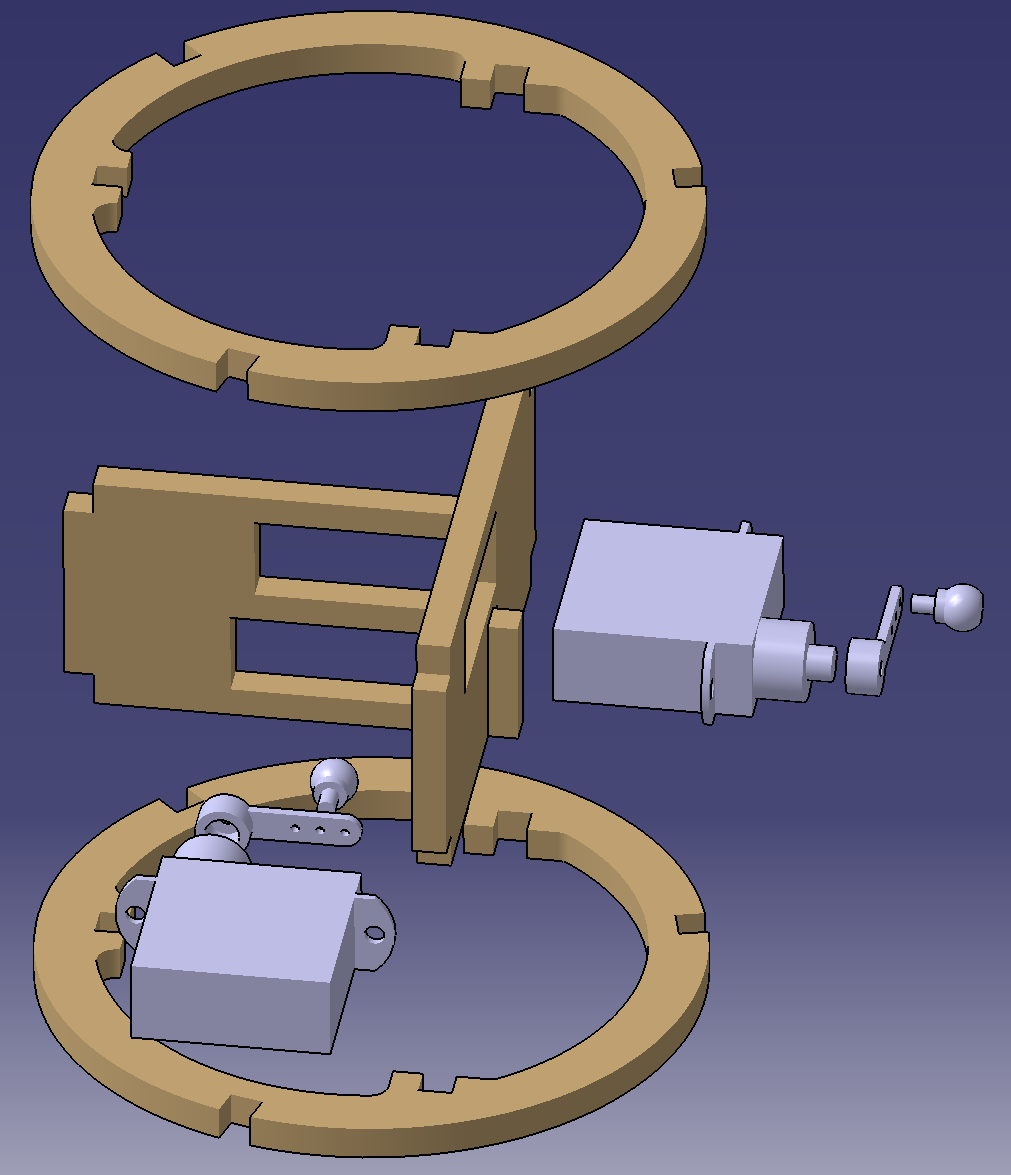
\includegraphics[height=75mm]{servo_1.png}\end{center}
\end{frame}

\begin{frame}{Servos montiert}
\begin{center}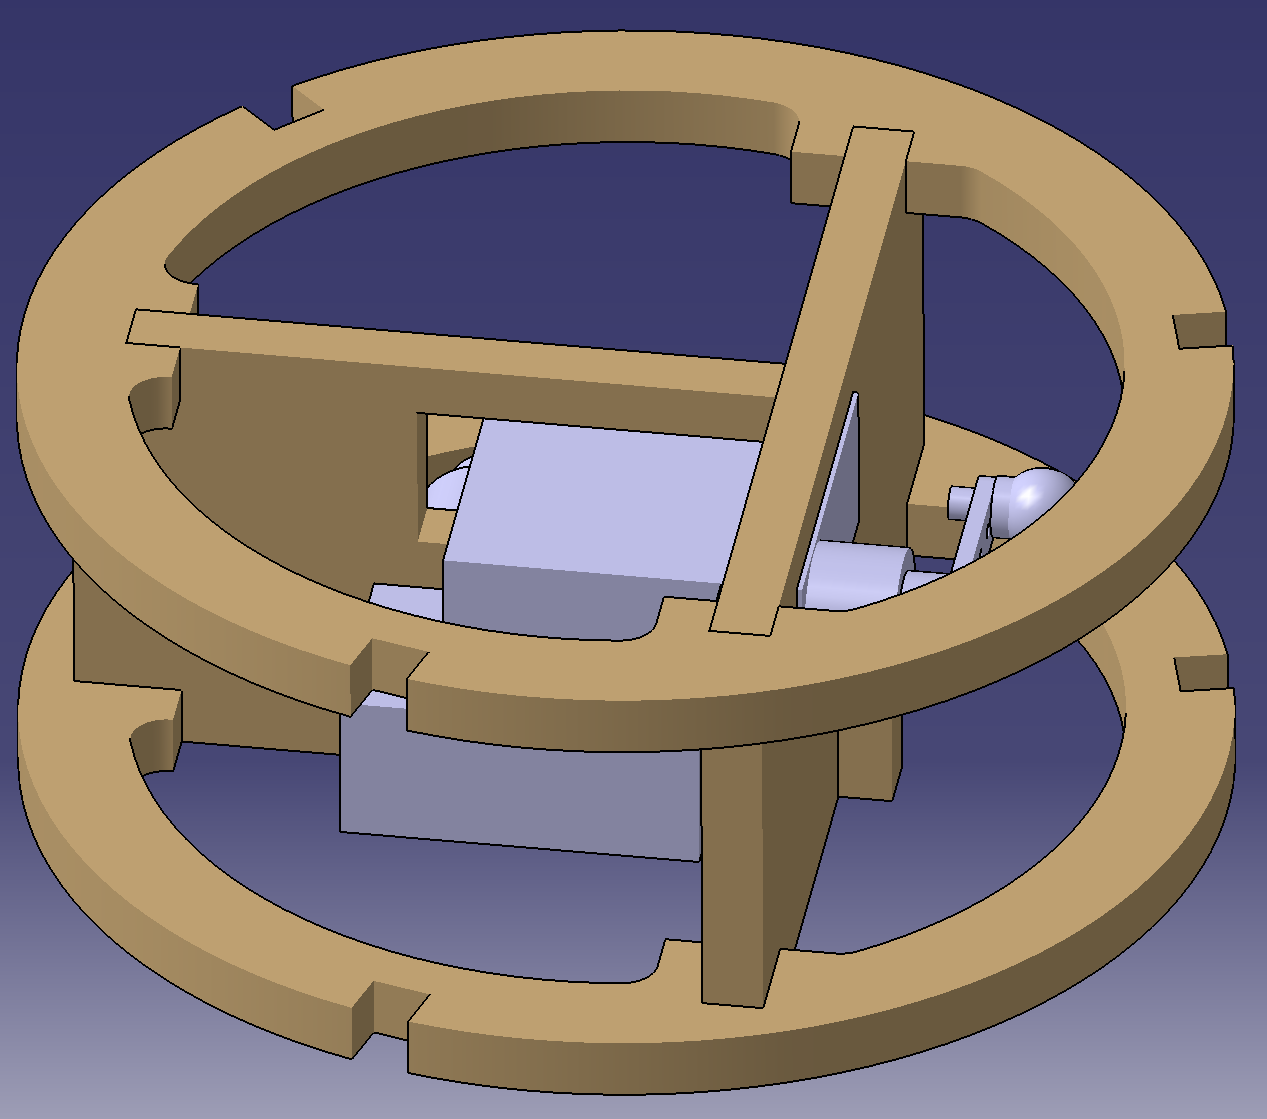
\includegraphics[height=75mm]{servo_2.png}\end{center}
\end{frame}

\begin{frame}{Servos und Motorhalterung}
\begin{center}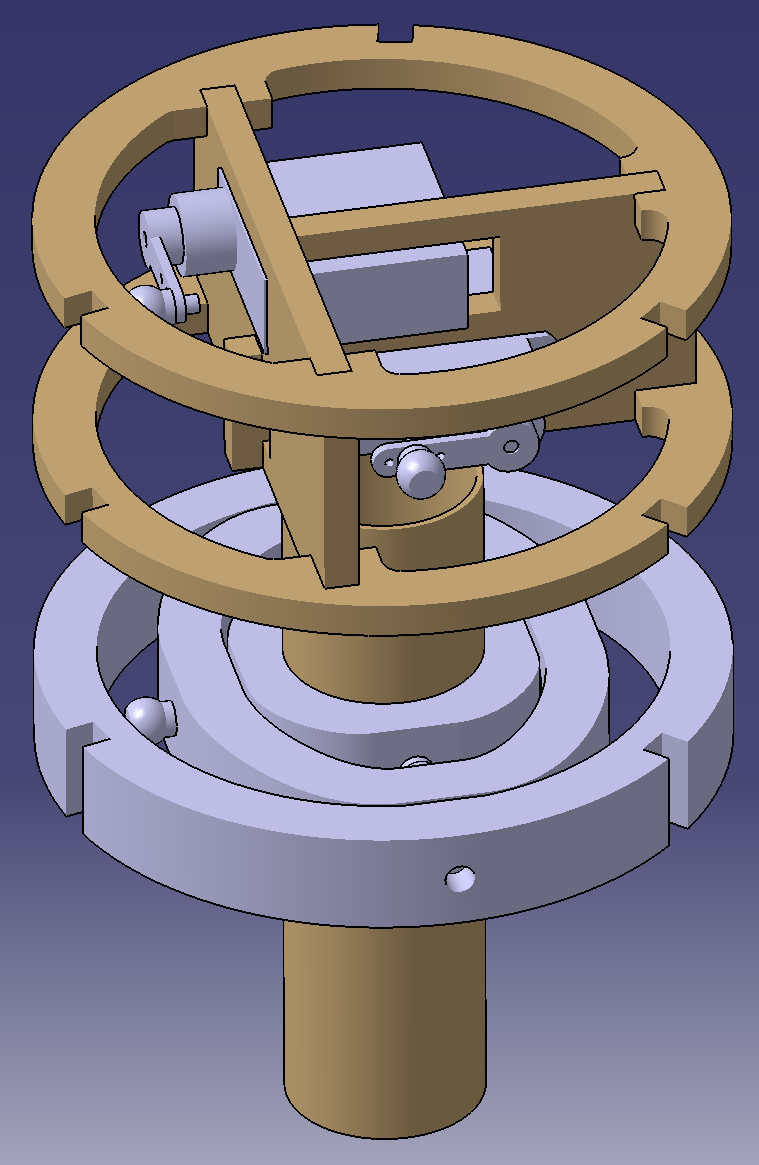
\includegraphics[height=75mm]{servo_3.png}\end{center}
\end{frame}

\begin{frame}{Stringer-Struktur}
\begin{center}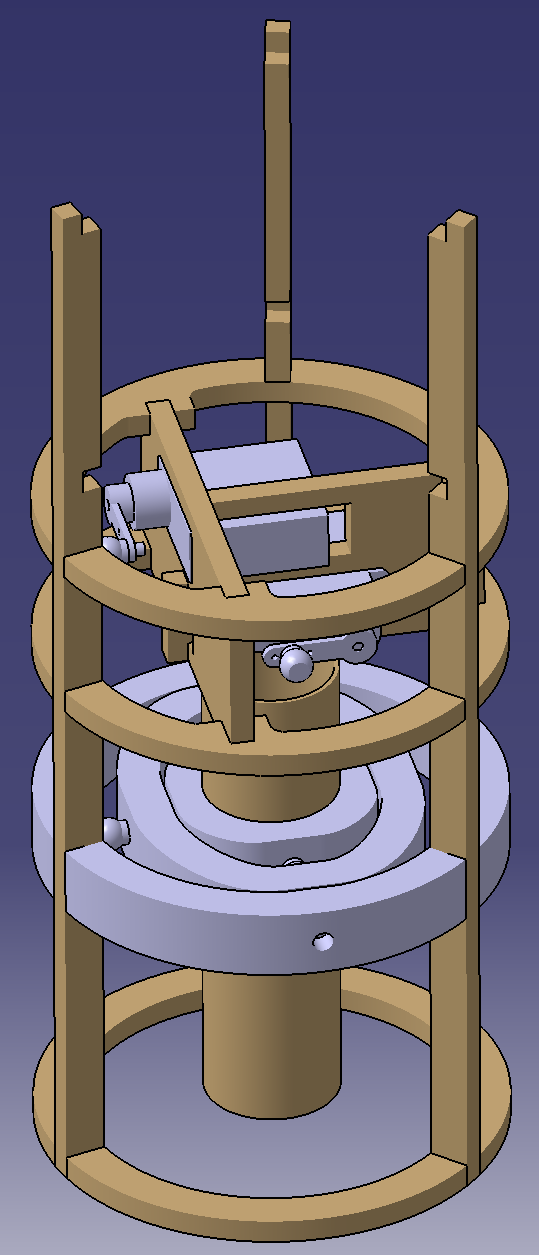
\includegraphics[height=75mm]{struktur_1.png}\end{center}
\end{frame}

\begin{frame}{Elektronik-Komponenten}
\begin{center}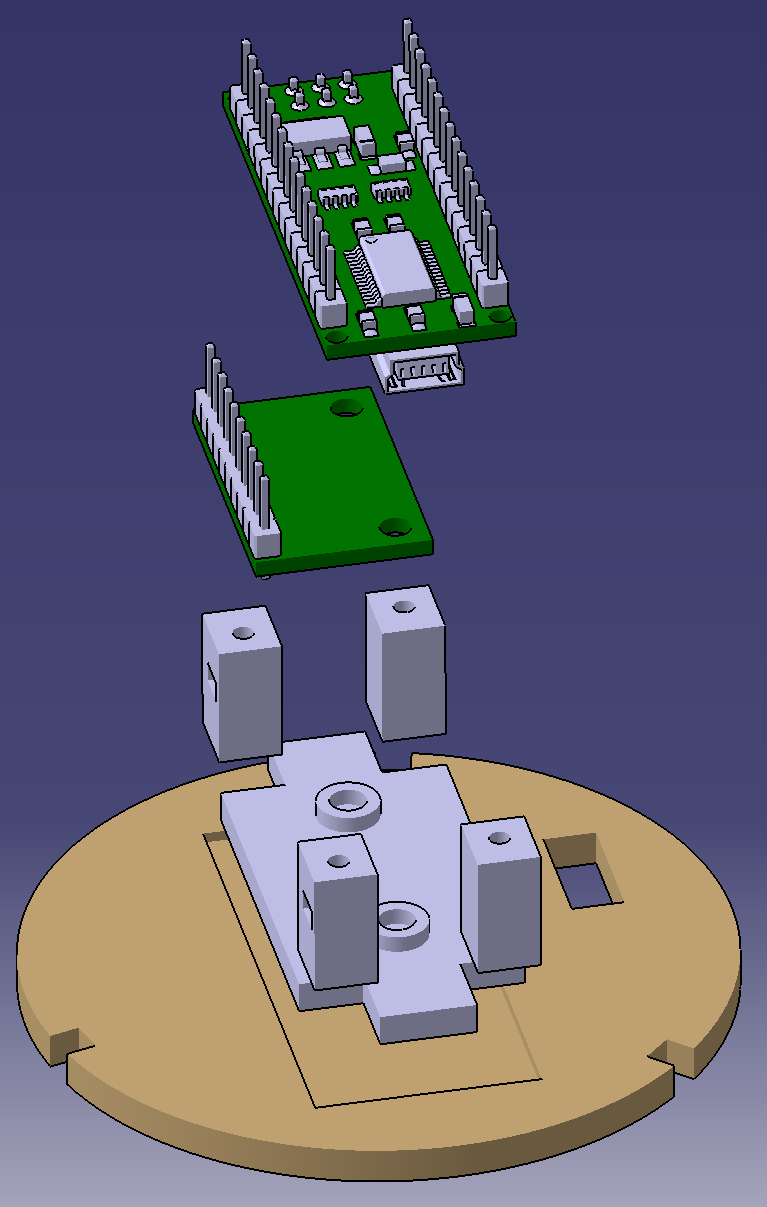
\includegraphics[height=75mm]{elektronik_1.png}\end{center}
\end{frame}

\begin{frame}{Elektronik montiert -- ohne Kabelsalat}
\begin{center}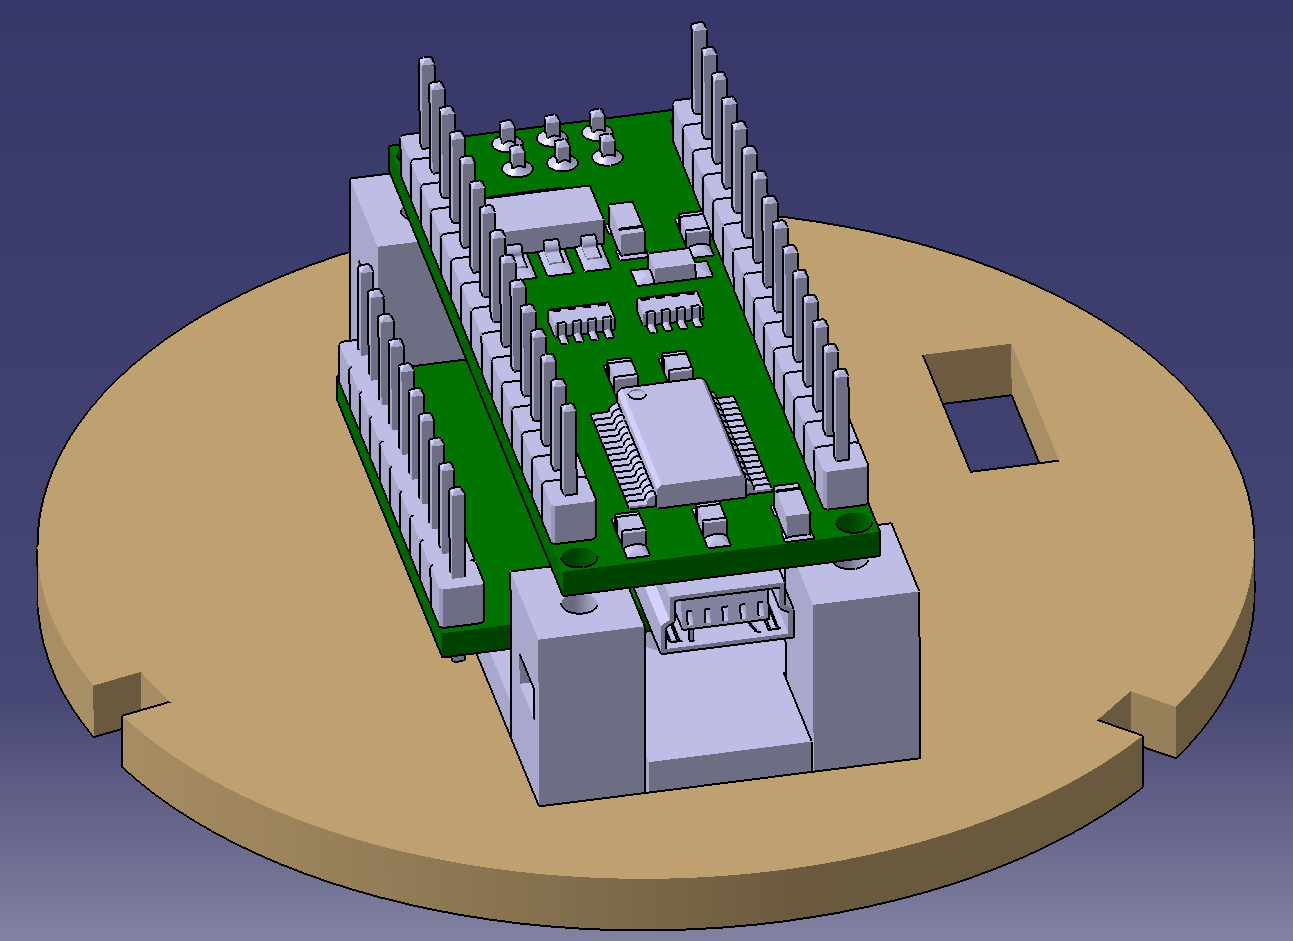
\includegraphics[height=75mm]{elektronik_2.png}\end{center}
\end{frame}

\begin{frame}{Struktur komplett}
\begin{center}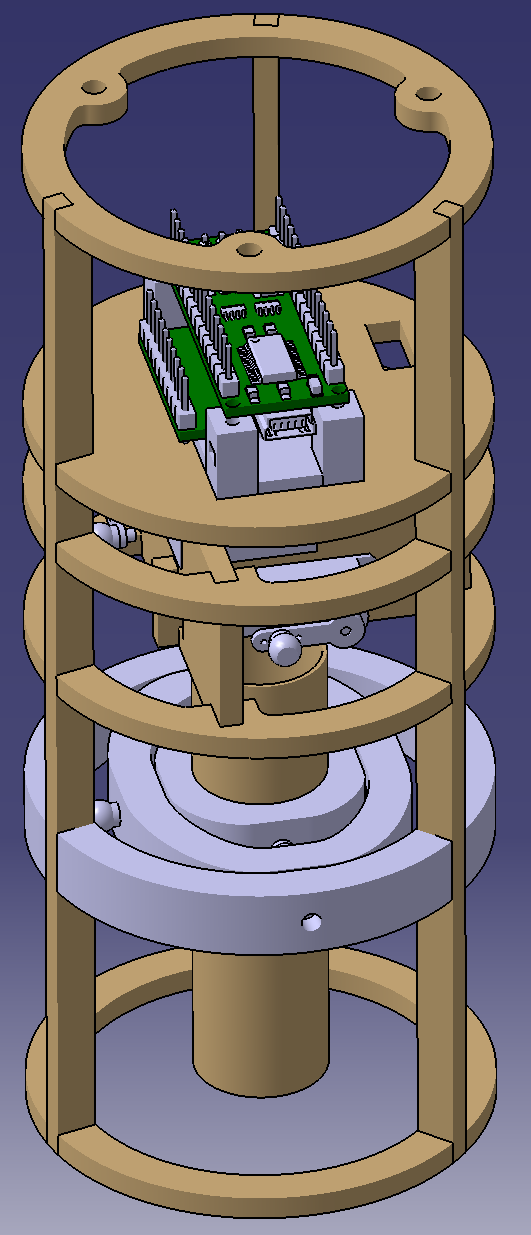
\includegraphics[height=75mm]{struktur_2.png}\end{center}
\end{frame}

\section{Elektronik}

\begin{frame}{Elektronik}
\begin{center}
\begin{tikzpicture}[auto,node distance=2cm,>=latex]
    \node [block] (bat) at (0,2) {Batterie};
    \node [block] (BEC) at (2,2) {BEC};
    \node [block] (uC) at (5,2) {Arduino Nano};
    \node [block] (IMU) at (8,2) {GY-80 IMU};
    \node [block] (ServoX) at (4,4) {Servo X};
    \node [block] (ServoY) at (6,4) {Servo Y};
    \node [block] (Eject) at (5,0) {Ausstoßladung};
    
    \draw (bat) -- (BEC);
    \draw (BEC) -- (uC);
    \draw (uC) -- (IMU);
    \draw (uC.south) -| (Eject.north);
    \draw (4,2.4) |- (4,3.6);
    \draw (6,2.4) |- (6,3.6);
    
    \draw [dotted] (BEC.north) |- (2,3) -| (3.5,3.6);
    \draw [dotted] (BEC.north) |- (2,3) -| (5.5,3.6);
    \draw [dotted] (BEC.south) |- (2,1) -| (4.5,0.4);
\end{tikzpicture}
\end{center}
\end{frame}

\section{Simulation}

\begin{frame}{Modellbildung}
\begin{center}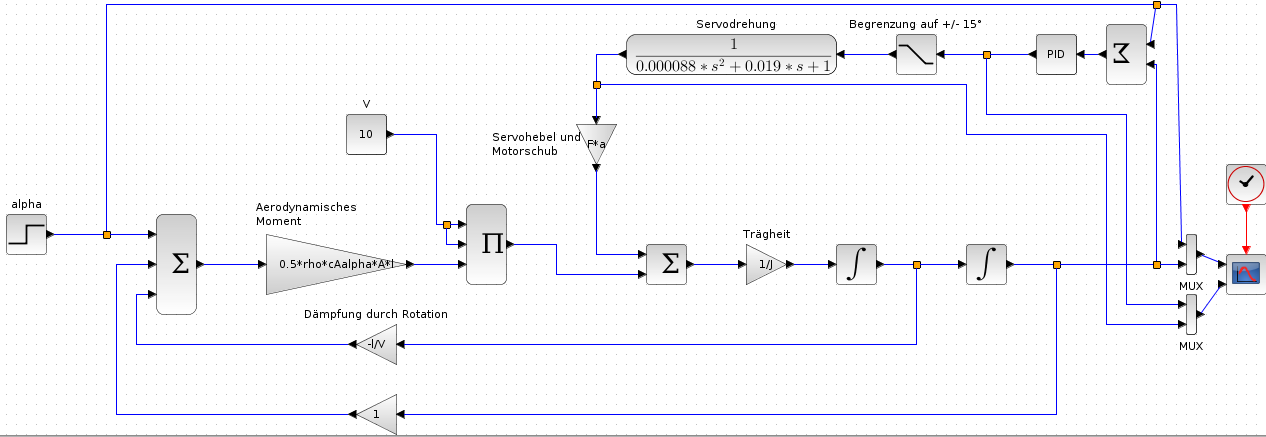
\includegraphics[width=\textwidth]{model.png}\end{center}
\end{frame}

\begin{frame}{Servoverhalten}
\begin{center}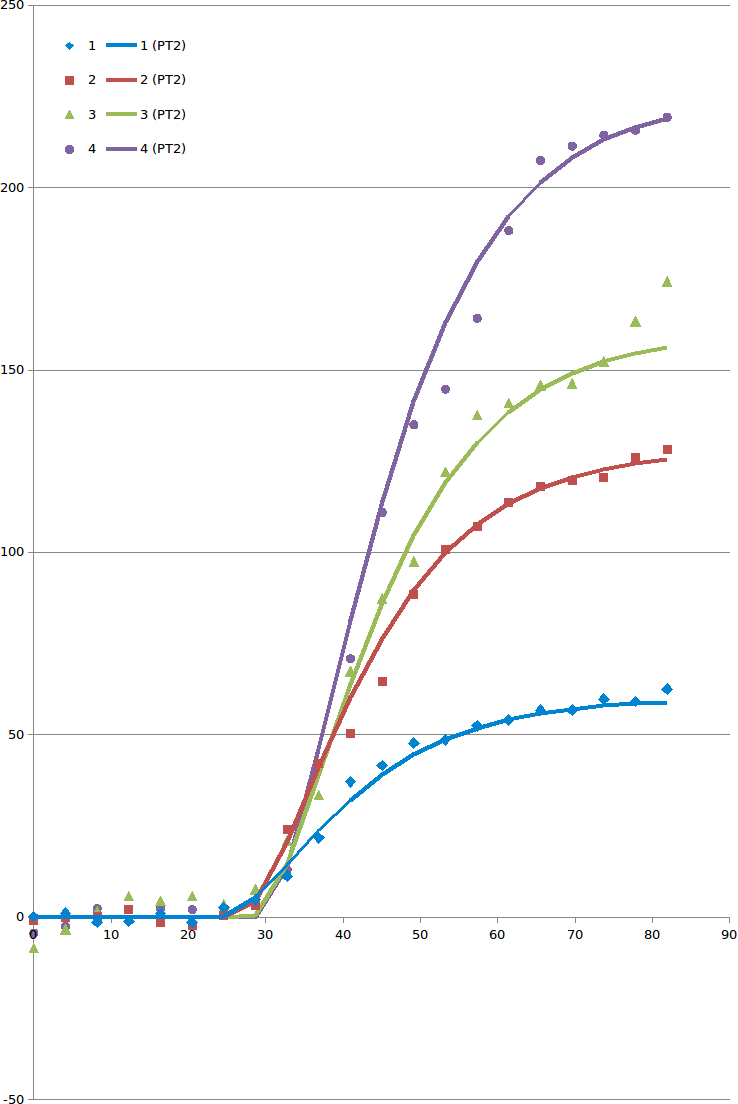
\includegraphics[height=75mm]{naeherung.png}\end{center}
\end{frame}

\begin{frame}{Vorhergesagte Reaktion auf Anstellwinkeländerung}
\begin{center}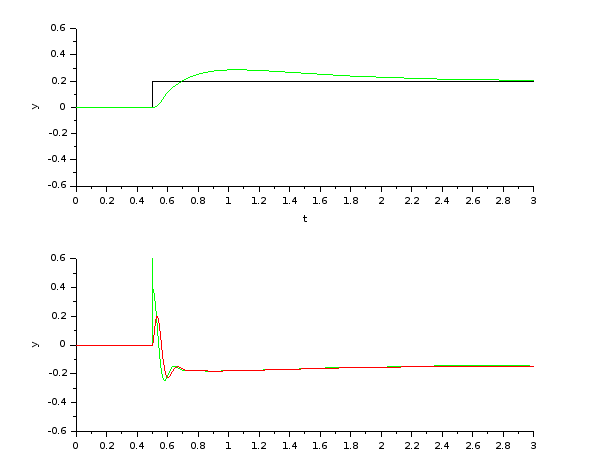
\includegraphics[height=70mm]{alpha_gamma.png}\end{center}
$K_P = 2,0;\quad K_I=1,8;\quad K_D = 0,3$
\end{frame}

\section{Firmware}

\begin{frame}{Firmware}
\begin{itemize}
\item State Machine mit drei Zuständen
\item Ausführen der einzelnen Operationen alle $10\u{ms}$ mittels Interrupt
\end{itemize}
\begin{enumerate}
\item \texttt{ON\_RAMP}
\begin{itemize}
\item Messung der Beschleunigung in $z$-Richtung
\item Messung der Drehraten um $x$- und $y$-Achsen
\item Laufende Bildung von Mittelwerten für alle Messgrößen für Korrektur der Werte im Flug
\item Überwachen der Beschleunigung, bei Überschreiten von $20\u{m/s^2}$ Wechsel zu \texttt{IN\_FLIGHT}
\end{itemize}
\seti
\end{enumerate}
\end{frame}

\begin{frame}{Firmware}
\begin{enumerate}
\conti
\item \texttt{IN\_FLIGHT}
\begin{itemize}
\item Flugzustandsschätzung mittels Kalman-Filter
\item Vorhersage, z. B. für Flughöhe \begin{eqnarray}\hat{h}_{i+1} &=& h_i + \Delta t\,v_i + \tfrac{1}{2} \Delta t^2\, a_i \\
\hat{v}_{i+1} &=& v_i + \Delta t a_i \\
\hat{a}_{i+1} &=& a_i \end{eqnarray}
\item Korrektur \begin{equation}a_{i+1} = (1-K_a) \hat{a}_{i+1} + K_a \tilde{a}\end{equation}
\item Kalman-Gains wurden offline mit simulierten Werten ermittelt
\item Berechnung der Soll-Position $u$ des Servos der jeweiligen Achse anhand des Fehlers
\begin{eqnarray}E_{\gamma} &=& E_{\gamma} + \Delta t\,\gamma \\
u &=& K_P\,\gamma + K_I\,E_{\gamma} + K_D\,\dot{\gamma}\end{eqnarray}
\item Wechsel zu \texttt{RECOVERY} wenn ein Bahnwinkel 90° überschreitet oder die Geschwindigkeit unter 0 fällt
\end{itemize}
\seti
\end{enumerate}
\end{frame}

\begin{frame}{Firmware}
\begin{enumerate}
\conti
\item \texttt{RECOVERY}
\begin{itemize}
\item Pin für Ausstoßladung für 1 Sekunde auf \texttt{HIGH} setzen
\item Servos auf Mittelposition stellen
\item Bis in alle Ewigkeit die LED blinken lassen ...
\end{itemize}
\end{enumerate}
\end{frame}

\section{Ergebnisse}

\begin{frame}{Probeflug}
Werdet Ihr gleich sehen ...
\end{frame}

\begin{frame}{Offene Fragen}
\begin{itemize}
\item Sind die Servos gut geeignet (Zittern)?
\item Ist die Motoransteuerung verbesserungsfähig?
\item Wie kann das Design vor allem hinsichtlich Montage verbessert werden?
\item Gibt es bessere (geeignete) Sensoren?
\item Ist der Kalman-Filter richtig eingestellt?
\item Muss der Regler besser eingestellt werden?
\end{itemize}
\end{frame}

\end{document}
